\chapter{Image Formation and Camera Models}
\label{ch:camera}
\chaptermark{Image Formation} % short running header

\begin{objectives}
\begin{itemize}
  \item Understand how a camera forms an image: pinholes, lenses, focus, sensors, exposure and shutters.
  \item Derive the pinhole projection, the intrinsic matrix and normalized image coordinates.
  \item Use homogeneous coordinates and the basic projective geometry of points, lines and homographies.
  \item Model and invert the radial-tangential lens distortion used by EuRoC, and know the fisheye alternative.
  \item Understand how cameras are calibrated.
  \item State the project's camera measurement model with its noise, derive the projection Jacobian, and understand extrinsics and time offsets.
\end{itemize}
\end{objectives}

% ==============================================================================
\section{How a camera forms an image}

\subsection{From pinhole to lens}

A camera measures the \emph{directions} of light rays. In a \emph{camera obscura}, light from the scene enters a dark box through a tiny hole and
forms an inverted image on the opposite wall: every point of the wall receives light only from the scene point on the straight line through the
hole. This is the \term{pinhole model}, and it is geometrically perfect. It is also impractical: a hole small enough to give a sharp image lets in
very little light.

A lens gathers light through a large aperture and bends it so that all rays from one scene point converge again at one image point. For an ideal
\emph{thin lens} of focal length $f_L$, a point at distance $z_o$ in front of the lens is imaged sharply at distance $z_i$ behind it, where
\begin{equation}
  \frac1{f_L} = \frac1{z_o} + \frac1{z_i} .
\end{equation}
For distant scenes ($z_o \gg f_L$) the image forms at $z_i \approx f_L$, which is where the sensor sits in a camera focused at infinity. Points at other
distances form slightly blurred spots; the range of distances that stays acceptably sharp is the \emph{depth of field}, larger for small apertures and
short focal lengths. The central ray through the lens center is not bent, so the geometry of a focused lens camera is exactly that of a pinhole at
the lens center: the pinhole model describes it, and lens imperfections are added as \emph{distortion} (\cref{sec:distortion}).

\subsection{The image sensor}

The sensor is a grid of light-sensitive \emph{pixels}. Each accumulates charge in proportion to the light it receives during the \emph{exposure time},
and the charge is converted into a number, typically 8 bits per pixel for the monochrome cameras of EuRoC. Several properties of the sensor matter to an
estimator.
\begin{itemize}
  \item \emph{Exposure and motion blur.} A camera rotating at $\omega$ rad/s during an exposure of $T$ seconds smears each point over about $f\omega T$ pixels, with
        $f$ the focal length in pixels. At 1~rad/s, 5~ms and $f = 458$~px this is 2.3~px, enough to degrade feature tracking. EuRoC's difficult
        sequences contain exactly such blur.
  \item \emph{Global versus rolling shutter.} A global shutter exposes all pixels at the same instant, as EuRoC's cameras do. A rolling shutter (common in
        phones) exposes rows one after another, so each row is captured at a different time and, on a moving camera, from a different pose. Rolling-shutter
        images need an extended measurement model.
  \item \emph{Noise and dynamic range.} Pixel values carry photon and electronic noise, and scenes brighter or darker than the sensor's range saturate. Auto
        exposure changes the brightness of the same scene point between frames, which matters for intensity-based tracking (\cref{ch:frontend}).
\end{itemize}

\paragraph{Pixel coordinates.} We write pixel coordinates as $(u, v)$, with $u$ increasing to the right and $v$ increasing downward, and the origin at the
top-left of the image. In OpenCV's convention, integer coordinates are pixel \emph{centers}. The camera frame $C$ is aligned with this: $x_c$ to the right, $y_c$
down, $z_c$ along the optical axis into the scene.

% ==============================================================================
\section{The pinhole projection}

An ideal pinhole camera lets light through a single point, the optical center. A scene point with camera-frame coordinates $p_c = (X, Y, Z)$, with $Z$ along the
optical axis, projects through the center onto an image plane. Placing a virtual image plane at unit distance \emph{in front of} the center (which avoids
the inversion of the physical image) and using similar triangles, the image of the point is
\begin{equation}
  \pi(p_c) = \begin{bmatrix} x \\ y \end{bmatrix} = \begin{bmatrix} X/Z \\ Y/Z \end{bmatrix}.
  \label{eq:pinhole}
\end{equation}
These are the \term{normalized image coordinates}: dimensionless, independent of the lens, and equal to the tangents of the ray's angles from the optical axis.
The vector $\bar x = (x, y, 1)$ is the \term{bearing} of the point, defined up to scale.

\begin{figure}[t]
\centering
\begin{tikzpicture}[scale=1.0]
  \coordinate (O) at (0,0);
  \draw[frameaxis, plotblue] (O) -- (6.2,0) node[right] {$z_c$ (optical axis)};
  \draw[frameaxis, plotorange] (O) -- (0,-1.6) node[below] {$y_c$};
  \fill (O) circle (1.6pt) node[above left] {$C$};
  \draw[thick, primary] (2,1.8) -- (2,-1.4);
  \node[primary, font=\footnotesize, align=center] at (2,2.15) {normalized plane $Z = 1$};
  \coordinate (P) at (5.6,-1.25);
  \fill[plotgreen] (P) circle (2pt) node[right] {$p_c = (X, Y, Z)$};
  \draw[plotgreen, dashed] (O) -- (P);
  \coordinate (I) at (2,{-1.25*2/5.6});
  \fill[conv] (I) circle (1.8pt);
  \node[conv, font=\footnotesize, right] at (2.05,-0.18) {$y = Y/Z$};
  \draw[<->, black!60] (0,0.5) -- (2,0.5) node[midway, above, font=\footnotesize] {$1$};
  \draw[<->, black!60] (0,0.95) -- (5.6,0.95) node[midway, above, font=\footnotesize] {$Z$};
\end{tikzpicture}
\caption{Pinhole projection in the $y$-$z$ plane. The ray from the optical center $C$ to the point intersects the plane $Z = 1$ at height $Y/Z$. All points
along the ray project to the same image point, so depth is lost.}
\label{fig:pinhole}
\end{figure}

\subsection{Intrinsic parameters}

Pixels are obtained by scaling and shifting the normalized coordinates with the \term{intrinsic matrix}:
\begin{equation}
  \begin{bmatrix} u \\ v \\ 1 \end{bmatrix} = K\begin{bmatrix} x \\ y \\ 1 \end{bmatrix}, \qquad
  K = \begin{bmatrix} f_u & s & c_u \\ 0 & f_v & c_v \\ 0 & 0 & 1 \end{bmatrix},
\end{equation}
with focal lengths $f_u, f_v$ in pixels, principal point $(c_u, c_v)$ (where the optical axis pierces the image), and skew $s$ (zero for modern sensors). The
focal length in pixels is the physical focal length divided by the pixel pitch; $f_u \neq f_v$ if pixels are not square. Inverting $K$ turns a pixel into a bearing,
$\bar x = K\inv(u, v, 1)\T$. The horizontal \emph{field of view} of a $W$-pixel-wide image is $2\arctan\big(W/(2f_u)\big)$, ignoring distortion. EuRoC's \code{cam0} has
$f_u = 458.654$, $f_v = 457.296$, $c_u = 367.215$, $c_v = 248.375$ on a $752\times480$ sensor: a horizontal field of view of about $79^\circ$.

% ==============================================================================
\section{Homogeneous coordinates and projective geometry}
\label{sec:homogeneous}

\subsection{Points and lines in the image}

\index{homogeneous coordinates}
The image point $(x, y)$ corresponds to the whole ray of 3D vectors $\lambda(x, y, 1)$, $\lambda \ne 0$. \term{Homogeneous coordinates} make this explicit: a point of the
plane is represented by any non-zero 3-vector $\tilde x = (x_1, x_2, x_3)$, with $\tilde x$ and $\lambda\tilde x$ representing the same point, and the ordinary coordinates
are recovered as $(x_1/x_3, x_2/x_3)$. Vectors with $x_3 = 0$ represent \emph{points at infinity}: directions, where parallel lines meet.

A line $ax + by + c = 0$ is represented by the 3-vector $l = (a, b, c)$, also up to scale, and a point lies on it exactly when
\begin{equation}
  l\T\tilde x = 0 .
\end{equation}
This symmetric relation makes two constructions one-liners:
\begin{itemize}
  \item the line through two points is $l = \tilde x_1\times\tilde x_2$ (it is orthogonal to both, so both lie on it);
  \item the intersection of two lines is $\tilde x = l_1\times l_2$ (by the same argument).
\end{itemize}
Two parallel lines $(a, b, c_1)$ and $(a, b, c_2)$ intersect at $(b, -a, 0)$ times a constant: a point at infinity in their common direction. In an image of a
3D scene, parallel 3D lines are generally not parallel in the image and meet at a finite \emph{vanishing point}, the image of their common direction.

\subsection{Homographies}

\begin{definition}[Homography]
\index{homography}
A \term{homography} (projective transformation) of the plane is a map $\tilde x \mapsto H\tilde x$ for an invertible $3\times3$ matrix $H$, defined up to scale (eight
degrees of freedom).
\end{definition}

Homographies map lines to lines (if $l\T\tilde x = 0$ then $(H\mT l)\T(H\tilde x) = 0$) but do not preserve parallelism, lengths or angles. Two situations in
which they arise are central to vision:
\begin{itemize}
  \item the images of a \emph{plane} in two views are related by a homography (\cref{ch:multiview}), which is the basis of camera calibration below;
  \item two images taken by a camera that only \emph{rotates} are related by the homography $KRK\inv$, independently of the scene (\cref{ch:multiview,ch:frontend}).
\end{itemize}

\subsection{The projection matrix}

In homogeneous coordinates the complete projection of a world point $p_w$ (with homogeneous coordinates $\tilde p_w = (p_w, 1)$) into pixels is a single linear map,
\begin{equation}
  \lambda\begin{bmatrix} u \\ v \\ 1\end{bmatrix} = K\begin{bmatrix} R_{cw} & p_{cw}\end{bmatrix}\tilde p_w = P\,\tilde p_w,
  \qquad P = K\,[R_{cw}\ \ p_{cw}] \in \R^{3\times4},
\end{equation}
where $(R_{cw}, p_{cw})$ maps world coordinates into the camera frame and $\lambda = Z$ is the depth. The \emph{camera matrix} $P$ has eleven degrees of freedom (twelve
entries up to scale): five intrinsic and six extrinsic. Linear methods that estimate $P$, $H$ or the essential matrix from correspondences
(\cref{ch:multiview}) all exploit the fact that projection is linear in homogeneous coordinates.

% ==============================================================================
\section{Lens distortion}
\label{sec:distortion}

Real lenses bend rays, most strongly near the image edges, so the image of a straight line is curved. The \term{radial-tangential} (Brown--Conrady) model
used by EuRoC maps ideal normalized coordinates $(x, y)$ to distorted ones $(x_d, y_d)$:
\begin{align}
  x_d &= x\,(1 + k_1r^2 + k_2r^4) + 2p_1xy + p_2(r^2 + 2x^2), \\
  y_d &= y\,(1 + k_1r^2 + k_2r^4) + p_1(r^2 + 2y^2) + 2p_2xy, \qquad r^2 = x^2 + y^2,
\end{align}
after which $K$ is applied to $(x_d, y_d)$. The \emph{radial} terms ($k_1, k_2$) model the dominant symmetric distortion of a lens; the \emph{tangential} terms ($p_1, p_2$)
model a lens slightly tilted or decentered relative to the sensor. For \code{cam0}, $(k_1, k_2, p_1, p_2) = (-0.2834, 0.07396, 1.94\times10^{-4}, 1.76\times10^{-5})$. The negative
$k_1$ produces \emph{barrel} distortion (\cref{fig:distortion}). At the middle of the left and right image edges the radial factor $1 + k_1r^2 + k_2r^4$ is about $0.79$,
which moves points by about 100 pixels; at the corners it is about $0.73$, a shift of about 160 pixels. Ignoring distortion is therefore not an option.

\begin{figure}[t]
  \centering
  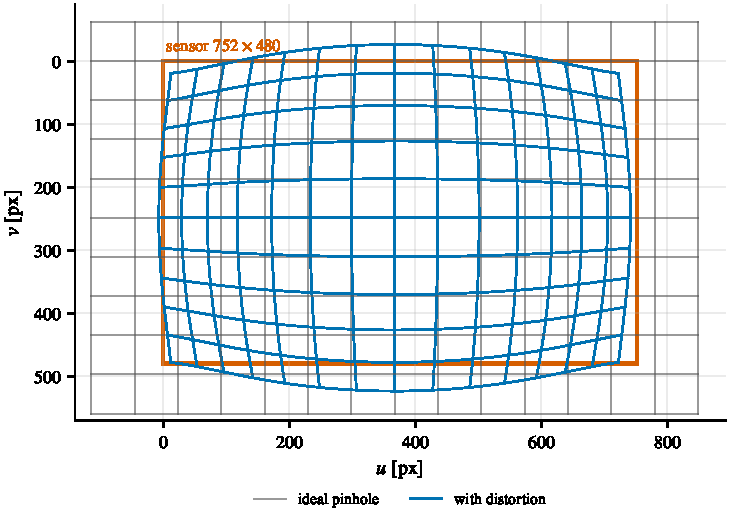
\includegraphics[width=0.84\textwidth]{fig_distortion.pdf}
  \caption{EuRoC \code{cam0} lens distortion. A regular grid in normalized coordinates (gray) is imaged by the real lens as the curved blue grid. Distortion pulls
  points toward the center, increasingly toward the edges, so the sensor (orange) sees a wider field than an ideal pinhole with the same focal length would.}
  \label{fig:distortion}
\end{figure}

\paragraph{Undistortion.} The front end measures distorted pixels and needs ideal normalized coordinates. The model has no closed-form inverse, but a fixed-point
iteration converges quickly for moderate distortion: starting from $x^{(0)} = x_d$,
\begin{equation}
  x^{(j+1)} = \frac{x_d - \Delta_x(x^{(j)}, y^{(j)})}{1 + k_1r_j^2 + k_2r_j^4},\qquad
  y^{(j+1)} = \frac{y_d - \Delta_y(x^{(j)}, y^{(j)})}{1 + k_1r_j^2 + k_2r_j^4},
\end{equation}
where $\Delta$ denotes the tangential terms. A Gauss--Newton iteration (\cref{ch:nlls}) with the $2\times2$ Jacobian of the distortion converges faster and more
reliably near the edges. OpenCV's \code{cv::undistortPoints} implements the iterative scheme. Milestone 8 checks undistortion by distorting and undistorting a
grid of points.

\begin{keyidea}[undistort points, not images]
The estimator needs a few hundred feature locations, not a rectified image. Undistorting only the tracked points costs microseconds; remapping a full image
costs milliseconds, resamples the pixels (blurring them), and changes the noise of the feature detector in a position-dependent way. Track in the raw image and
undistort the tracks.
\end{keyidea}

\paragraph{Wide-angle lenses.} Beyond about $120^\circ$ of field of view, the pinhole model itself breaks down (a ray at $90^\circ$ from the axis would have infinite
normalized coordinates). \emph{Fisheye} models parameterize the image radius as a function of the angle $\vartheta$ of the incoming ray, for example the
equidistant (Kannala--Brandt) model $r_d = \vartheta(1 + k_1\vartheta^2 + k_2\vartheta^4 + \cdots)$. The rest of the pipeline is unchanged: everything downstream of
undistortion works with bearings, which can be represented as unit vectors when they are far from the optical axis.

% ==============================================================================
\section{Camera calibration}

How were EuRoC's intrinsics and distortion coefficients obtained? By observing a known calibration target (a checkerboard or grid of markers) in many
images and fitting the camera model to the observed corner positions.

\paragraph{Zhang's method.} Place the target in the plane $Z = 0$ of its own frame. A target point $(X, Y, 0)$ then projects as
$\lambda\tilde u = K[r_1\ r_2\ r_3\ t](X, Y, 0, 1)\T = K[r_1\ r_2\ t](X, Y, 1)\T$: each image of the target is a homography $H = [h_1\ h_2\ h_3] \propto K[r_1\ r_2\ t]$, estimable from
four or more corner correspondences (\cref{ch:multiview}). Because $r_1$ and $r_2$ are orthonormal, $r_1 = \lambda K\inv h_1$ and $r_2 = \lambda K\inv h_2$ give two
constraints on the matrix $\omega = K\mT K\inv$:
\begin{equation}
  h_1\T\omega h_2 = 0, \qquad h_1\T\omega h_1 = h_2\T\omega h_2 .
\end{equation}
These are linear in the entries of the symmetric $\omega$, so three or more images determine it; $K$ follows from a Cholesky factorization of $\omega$. The linear
estimate is then refined, together with the distortion coefficients and each image's pose, by Levenberg--Marquardt (\cref{ch:nlls}) minimizing the
\emph{reprojection error}, the distance between observed and predicted corners. The residual reprojection error after calibration, typically a few tenths of a
pixel, is the standard measure of calibration quality.

\paragraph{Camera--IMU calibration.} The extrinsics $T_{bc}$ and the time offset are calibrated jointly with the IMU, by moving the rig in front of the target
(\cref{ch:imu}).

% ==============================================================================
\section{The measurement model}

\begin{convention}[camera model, AGENTS.md C6]
In normalized, undistorted image coordinates,
\begin{equation}
  p_c = R_{bc}\T\big(R_{wb}\T(p_f - p_{wb}) - p_{bc}\big), \qquad
  z = \begin{bmatrix} p_{c,x}/p_{c,z} \\ p_{c,y}/p_{c,z} \end{bmatrix} + n_{uv},
  \qquad \sigma_{uv} \approx \sigma_{px}/f .
\end{equation}
\end{convention}

The first equation chains the world-to-body and body-to-camera transformations of \eqref{eq:world-to-camera}. The noise model follows from $u = f_u x + c_u$: a pixel
error $\delta u$ corresponds to a normalized error $\delta u/f_u$. With $\sigma_{px} = 1$~px and $f \approx 458$~px, $\sigma_{uv} \approx 2.2\times10^{-3}$. Strictly, distortion makes the
mapping from pixel noise to normalized noise position-dependent, by the inverse of the distortion Jacobian, and $f_u \neq f_v$. Both effects are small for EuRoC and
conventionally ignored, but they are a legitimate refinement.

% ==============================================================================
\section{The projection Jacobian}

\begin{proposition}[Jacobian of the pinhole projection]
\label{prop:proj-jacobian}
\begin{equation}
  \frac{\partial\pi}{\partial p_c} = \frac{1}{Z}\begin{bmatrix} 1 & 0 & -X/Z \\ 0 & 1 & -Y/Z \end{bmatrix}
  = \frac1Z\begin{bmatrix} I_2 & -\pi(p_c) \end{bmatrix}.
\end{equation}
\end{proposition}
\begin{proof}
Differentiate $X/Z$ and $Y/Z$ with the quotient rule: $\partial(X/Z)/\partial X = 1/Z$, $\partial(X/Z)/\partial Z = -X/Z^2$, and similarly for $Y/Z$.
\end{proof}

The Jacobian has rank two, and its nullspace is spanned by $p_c$ itself: moving the point along its viewing ray does not change its image. This is the single-view
loss of depth in differential form, and it is why a feature must be observed from at least two sufficiently different viewpoints before it constrains anything
(\cref{ch:multiview}). The factor $1/Z$ says that distant points have small image motion for a given change in position. They constrain rotation well and
translation poorly.

The full measurement Jacobian with respect to the filter state is the chain-rule product of this matrix with the Jacobian of $p_c$ with respect to the clone pose
and the feature position. Deriving those is part of \cref{ch:msckfupdate}.

\begin{pitfall}[points behind the camera]
\eqref{eq:pinhole} happily projects points with $Z < 0$, flipping their image through the center. A triangulation or linearization that produces a negative depth must
be rejected (the \emph{cheirality} check), not projected. Points with very small positive $Z$ produce huge Jacobians and should be rejected too.
\end{pitfall}

% ==============================================================================
\section{Extrinsics and time offset}

\paragraph{Extrinsic calibration.} The transformation $T_{bc}$ between the IMU and the camera is estimated offline, for EuRoC with Kalibr~\cite{furgale2013kalibr}, and
stored as \code{T\_BS} in \code{cam0/sensor.yaml}. Its rotation is close to a permutation of axes, and its translation is a few centimeters (\cref{app:euroc}). An error of
$\delta\phi$ in the extrinsic rotation biases every predicted bearing by about $\delta\phi$, which looks to the filter like a systematic residual. A translation error matters
mostly for near points. The project treats $T_{bc}$ as exact (AGENTS.md C3). Estimating it online is a stretch goal.

\paragraph{Time offset.} If the camera timestamp differs from the IMU clock by $t_d$, a feature moving across the image at velocity $\dot z$ is measured with an error of
about $\dot z\,t_d$. A 1~ms offset at an image-plane velocity of 0.5 normalized units per second (fast rotation) is an error of $5\times10^{-4}$, a quarter of a pixel.
EuRoC is hardware synchronized, so $t_d \approx 0$; consumer devices can have offsets of tens of milliseconds and must estimate it online~\cite{li2014timeoffset}.

\begin{takeaways}
\begin{itemize}
  \item A focused lens camera has the geometry of a pinhole at the lens center; lens imperfections are modeled as distortion.
  \item Exposure time causes motion blur of about $f\omega T$ pixels; EuRoC's global shutter exposes all pixels at once.
  \item Normalized coordinates $(X/Z, Y/Z)$ are lens-independent bearings; $K$ maps them to pixels.
  \item Homogeneous coordinates make projection linear; lines through points and intersections of lines are cross products; homographies map planes and pure
        rotations between views.
  \item EuRoC's lens has strong barrel distortion; undistort the tracked points, not the images.
  \item Cameras are calibrated by fitting the model to images of a known target, minimizing reprojection error.
  \item $\partial\pi/\partial p_c = \frac1Z[I_2\ \ {-\pi(p_c)}]$; its nullspace is the viewing ray.
\end{itemize}
\end{takeaways}

\begin{exercises}
  \item A lens with $f_L = 4$~mm is focused at infinity. How far must the sensor move to focus on an object at 0.5~m?
  \item Compute the horizontal and vertical fields of view of \code{cam0} with and without distortion.
  \item Compute the intersection of the lines $x + y = 1$ and $x - y = 0$ with homogeneous coordinates, and the line through $(1, 2)$ and $(3, 1)$.
  \item Show that two parallel lines intersect at a point at infinity, and find the vanishing point of the image of a family of parallel 3D lines with
        direction $d$ under the camera $P = K[I\ \ 0]$.
  \item Implement distortion and fixed-point undistortion for the EuRoC model. How many iterations are needed for $10^{-6}$ accuracy at the image corners? Compare
        with Gauss--Newton.
  \item Derive the two linear constraints of Zhang's method from the orthonormality of $r_1$ and $r_2$.
  \item A point at depth 10~m is observed by a camera translating sideways at 1~m/s and rotating at 1~rad/s. Which motion dominates its image velocity? What does
        this imply for the observability of translation from distant points?
\end{exercises}
